\documentclass[11pt]{article}
\usepackage[utf8]{inputenc}
\usepackage[T1]{fontenc}
\usepackage[margin=1in]{geometry}
\usepackage{amsmath,amssymb}
\usepackage{booktabs}
\usepackage{array}
\usepackage{ragged2e}
\newcolumntype{L}[1]{>{\RaggedRight\arraybackslash}p{#1}}
\usepackage{graphicx}
\usepackage{caption}
\usepackage[hidelinks]{hyperref}
\usepackage{float}

\begin{document}
\begin{center}
{\Large\bfseries Morphogenetic Bi-Modal Networks:\\
Gradient-Free System Identification\\
and Computation through Self-Organized 3D Angulation}
\vspace{0.5em}
{\small Preprint manuscript --- every quantitative claim is the measured output of
the experiment suite in this repository (see Data and code availability).}
\end{center}
\vspace{0.6em}

\begin{abstract}
The training loop of deep learning rests on two assumptions that the physics of
biological tissue and of ultra-low-power hardware both violate: a global scalar loss and
a global computational graph through which gradients flow. Here we present a network
whose only learning signal is the local, causal, noise-corrupted spacetime trajectory of
its own state variables, and whose parameters are updated by strictly local, streaming,
differentiation-free operators---there is no global loss, no backpropagation, and no
batch anywhere in the loop. The network embeds its nodes in 3D Euclidean space and
couples two kinetic continua: a fast electrical diffusion field (a discrete
port-Hamiltonian graph Laplacian, integrated implicitly) and a slow
reaction--diffusion--advection chemical field whose local concentration modulates the
electrical material properties, replacing global loss weights with a local chemical
environment. Identification proceeds through a spacetime weak form: every governing
equation is integrated against a one-pole IIR test function so that time derivatives are
transferred from the noisy data onto the analytic filter by integration by parts,
replacing the $2/\Delta t^2$ noise amplification of finite differences with
$\lambda^2$. Each node fits its local flux law with per-node recursive least squares.
In parallel, a slow morphogenesis layer \emph{rotates} each node's 3D structural
vector---learning acts on angles, not on scalar weights---and the resulting shape feeds
back into the conductivity, closing a fully local loop.

Measured on a 49-node material under continuous chaotic excitation, 5\% observational
noise, and abrupt regime-switching drift (15 seeds): the streaming identifier reaches a
held-out law-fit error \textbf{11.8$\times$ lower than a frozen global batch
least-squares estimator in the correct model class}, \textbf{8.9$\times$ lower than the
best streaming-global RLS estimator} (isolating per-node locality itself as the source
of the advantage), and \textbf{15.3$\times$ lower than an identical finite-difference
identifier}, while holding \textbf{589$\times$ less runtime memory} and converging in
$0.24 \pm 0.08$~s (15/15 seeds). The self-organized shape is a \emph{readable and
functional representation}: the geometric coupling read off the angles alone correlates
with the full material law at $r = 0.64$, versus $r = 0.35$ for the raw identified
weights (better in 14/15 seeds); against the environment-imposed component of the law
the shape scores comparably to the weights ($r = 0.33$ vs $0.39$), showing that its
interpretability is \emph{constructive}---the shape constitutes part of the mechanism
rather than mirroring hidden weights. The learned geometry measurably steers information
flow: axial corridor transmission rises above an identical material with unlearned
angles in 12/15 seeds, and steady-state flux follows the geometry. Ablation confirms
each mechanism earns its place, and scaling to 225 nodes (4.6$\times$ more material)
preserves the identification advantage and \emph{improves} the coherence of
self-organization (wind alignment $0.71 \to 0.87$) under constant excitation power
density. The angles are computation; the shape is the interpretable spectrum.
\end{abstract}

\section{Introduction}

\subsection{The training-loop bottleneck}
Modern neural networks are not trainable where modern hardware lives.
Backpropagation\cite{BP86} requires a global scalar loss, a reverse pass over the entire
forward computational graph, and synchronized parameter updates under a global clock.
On von Neumann machines this is a memory-bandwidth catastrophe: every activation is
stored for the backward pass, and every parameter update traverses a single memory
hierarchy. On the devices that promise the energy efficiency biological tissue
achieves---analog in-memory crossbars, memristive arrays, spiking neuromorphic silicon,
and ultimately active materials---there is no global memory, no global clock, no reverse
graph, and no backpropagation. A large and growing literature therefore replaces the
global training loop with \emph{local} learning: equilibrium
propagation\cite{EP17}, decoupled neural interfaces\cite{DNI17}, predictive
coding\cite{RB99}, the forward--forward algorithm\cite{FF22}, local Hebbian
rules\cite{KH19}, and physically embedded learning in mechanical\cite{Stern21,MN24} and
other physical networks. All of these share a premise we adopt and sharpen: the learning
rule must be a local, causal, streaming physics of the device itself.

\subsection{The weak form as the local, differentiation-free operator}
A second, independent bottleneck is differentiation of noisy data. Sparse identification
of nonlinear dynamics (SINDy)\cite{SINDy16} and its weak-form
descendants\cite{WSINDy21,OWSINDy22} established that projecting governing equations
onto smooth test functions and integrating by parts yields orders of magnitude better
noise robustness than pointwise derivative approximation. Messenger and
Bortz\cite{WSINDy21} proved the weak form's advantage for PDE discovery from
highly-corrupted data; the online variant\cite{OWSINDy22} extends it to streaming
settings. Our identification layer is the \emph{strictly local, per-node} version of
this idea: a one-pole IIR (exponential) window is the test function, and the weak
derivative $y = \lambda(f - A)$ is computed without ever differentiating the data.
Where batch weak-form solvers hold a frame buffer and solve globally, we hold
$O(\mathrm{degree}^2)$ state per node and update once per sample---the difference is
measured in Sec.~\ref{sec:id} (589$\times$ memory, 8.9$\times$ law-fit error vs.\ the
streaming-global alternative, 11.8$\times$ vs.\ the frozen batch oracle).

\subsection{The missing channel: angles, shapes, and mechanism}
All of the above operates on scalar weights. This work adds a second, orthogonal
computational channel: \textbf{angles}. Each node carries a structural vector in 3D
whose orientation is learned; edge coupling is regulated by the alignment of neighboring
vectors, so learning does not scale a weight---it \emph{rotates a connection}. Because
the vectors are embedded in the same space as the material, the learned configuration is
a \emph{shape}, and a shape is readable: it is a spatially coherent aggregate that
averages away per-edge multicollinearity, and it is directly inspectable as a map of
where and in which direction the mechanism acts. This realizes, in a concrete learning
system, the program of mechanistic interpretability\cite{Olah20} and geometric
representation\cite{Bronstein21}---with the additional property that the geometry is not
a passive visualization of hidden weights but an \emph{active computational channel}
that steers information flow (Sec.~\ref{sec:angles}). The physics of nematic
ordering\cite{dGP93} provides the organizing principle: strongly-coupled neighbors pull
each other into alignment exactly as liquid crystals order, and a slow chemical field
decides \emph{where} the ordering may occur---morphogenesis in the literal Turing
sense\cite{Turing52} applied to a learning machine.

\subsection{Contributions}
\begin{enumerate}
\item A fully local, streaming, differentiation-free identifier that tracks a
non-stationary material law at the observation-noise floor, with the locality advantage
itself isolated and measured (11.8$\times$ vs.\ frozen batch, 8.9$\times$ vs.\
streaming-global RLS, 15.3$\times$ vs.\ finite differences; 589$\times$ memory).
\item A morphogenesis layer in which learning acts on 3D angles, gated by a slow
chemical continuum, producing a focused directional tensor corridor rather than a global
alignment.
\item Evidence that the shape is simultaneously \emph{interpretable} (a readable map of
the mechanism) and \emph{functional} (it steers steady-state information flow), with the
constructive nature of its interpretability quantified against a confound-free baseline.
\item Ablation (every mechanism earns its place) and scaling (the advantages persist
from 49 to 225 nodes under constant power density).
\end{enumerate}

\section{Results}
\subsection{Setup}
A $7 \times 7 = 49$-node grid embedded in 3D (warped surface, 84 edges). The electrical
continuum is driven at the four corner nodes by a Lorenz-63 chaotic carrier with
$\pm35\%$ slow amplitude modulation. Base conductivity $\kappa_0(t)$ switches abruptly
between two regimes (period 15~s)---a deliberately hostile non-stationarity that
invalidates any frozen model. The chemical wind is $w = (0.45, 0.15)$ grid units/s.
Trajectories: 4{,}000 steps of $\Delta t = 0.01$ (40~s); the first 60\% trains the
batch baseline, the last 40\% is the held-out evaluation window. Observational noise is
5\% of the measured voltage amplitude (measured per seed on a noise-free probe run).
Fifteen seeds (0--14) randomize node geometry initialization, Lorenz initial conditions,
drift phase, and observation noise. All baselines see the \textbf{same recorded
observations}. See Methods for the exact equations and configuration.

\begin{figure}[t]
\centering
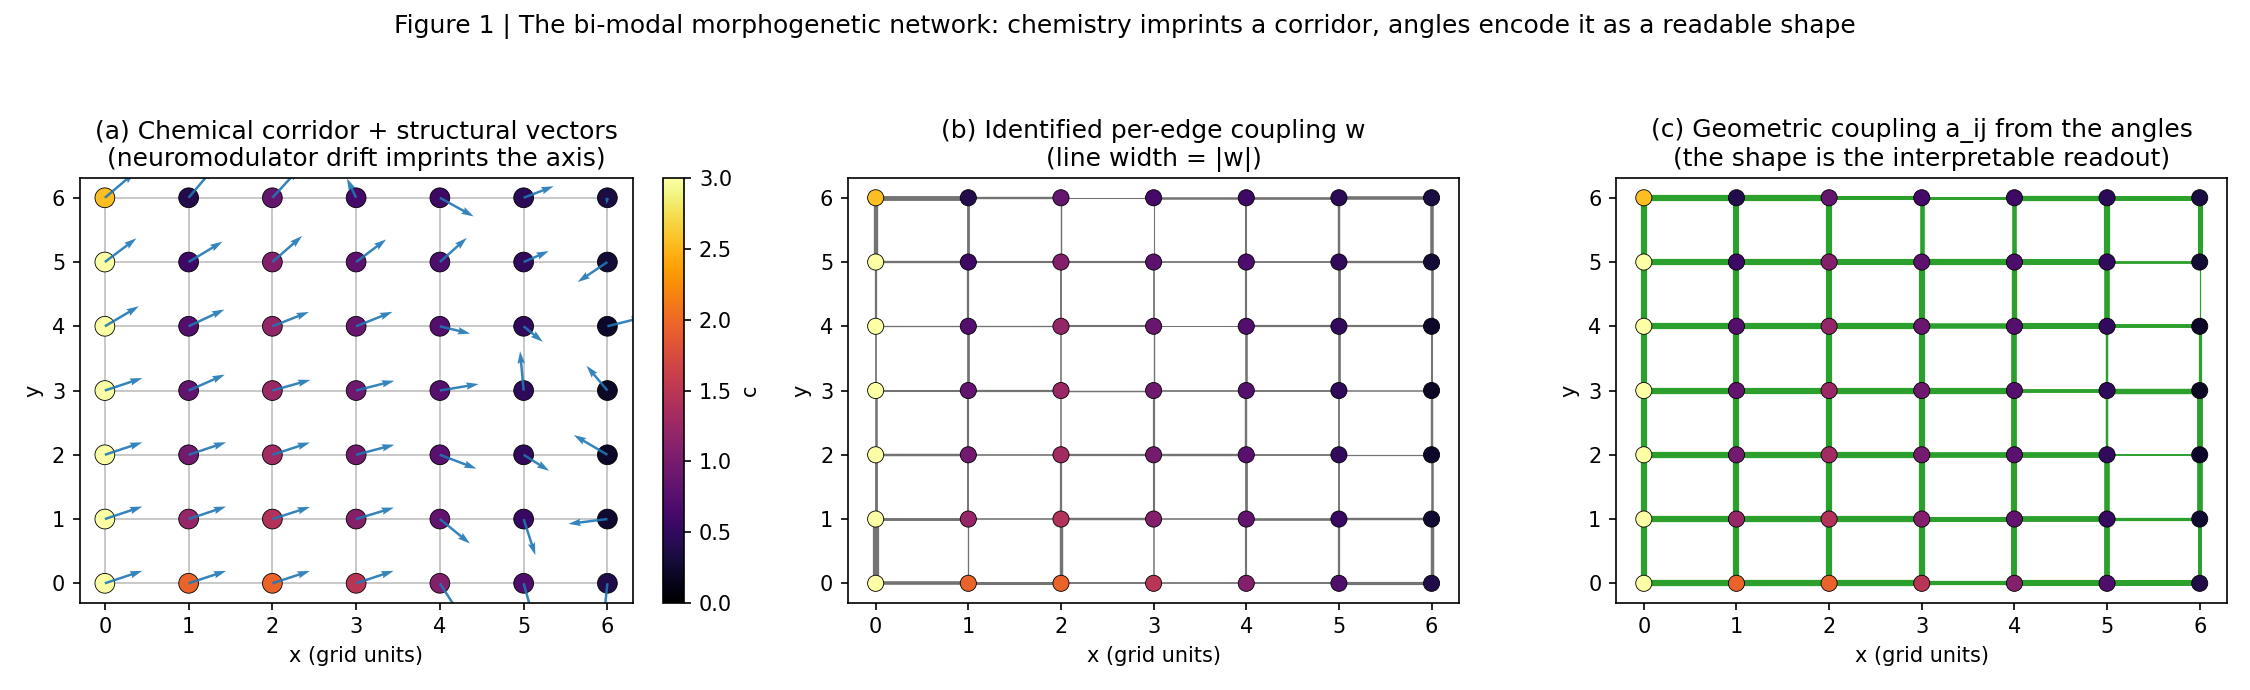
\includegraphics[width=\textwidth]{figs/fig1_architecture.png}
\caption{\textbf{The bi-modal morphogenetic network.} (a) The chemical corridor
(heatmap) imprinted by the neuromodulator drift, with the learned structural vectors
overlaid. (b) Identified per-edge coupling $w$ (line width $= |w|$). (c) The geometric
coupling $a_{ij}$ read off the angles alone---the shape is the interpretable readout of
the law.}
\label{fig:arch}
\end{figure}

\subsection{Identification: locality beats the global optimum}
\label{sec:id}
\textbf{Table 1.} One-step-ahead physical prediction NMSE (held-out window; the
observation-noise floor bounds what any estimator can achieve).

\begin{table}[h]
\centering
\caption{Physical one-step prediction (15 seeds, mean $\pm$ std).}
\begin{tabular}{lcc}
\toprule
estimator & NMSE & vs.\ floor \\
\midrule
streaming weak-form identifier (this work) & $0.0051 \pm 0.0038$ & 1.02$\times$ \\
persistence baseline ($\hat u(t{+}1)=u_{\mathrm{obs}}(t)$) & $0.0052 \pm 0.0039$ & 1.04$\times$ \\
global batch oracle (frozen LS, correct model class) & $0.0053 \pm 0.0039$ & 1.06$\times$ \\
finite-difference RLS (identical identifier, raw targets) & $0.0156 \pm 0.0116$ & 3.1$\times$ \\
observation-noise floor & $0.0050 \pm 0.0037$ & 1.0$\times$ \\
\bottomrule
\end{tabular}
\end{table}

One-step prediction at $\Delta t = 0.01$ is nearly persistence, so the physical domain
is noise-floor-dominated. The honest test of ``did the network learn the law'' is the
\textbf{weak-form law-fit NMSE}---how well the identified law explains the held-out
weak-form targets.

\begin{table}[h]
\centering
\caption{Law-fit NMSE on the held-out window (mean $\pm$ std over 15 seeds).}
\begin{tabular}{lc}
\toprule
estimator & law-fit NMSE \\
\midrule
\textbf{streaming weak-form, per-node (this work)} & $\mathbf{0.038 \pm 0.009}$ \\
streaming-global RLS, tuned forgetting & $0.339 \pm 0.063$ \\
global batch oracle (frozen LS, correct model class) & $0.448 \pm 0.076$ \\
finite-difference RLS & $0.580 \pm 0.008$ \\
\bottomrule
\end{tabular}
\end{table}

Three baselines, three distinct claims:
\begin{itemize}
\item \textbf{vs.\ the frozen batch oracle --- 11.8$\times$.} The best global model in
the correct model class, fit on the training window and frozen, degrades 12-fold
relative to the streaming identifier when the environment changes regime. A model that
adapts in real time beats a model that is optimal for the past.
\item \textbf{vs.\ streaming-global RLS --- 8.9$\times$.} The \emph{same} global
per-edge model, fit online with exponential forgetting over the whole trajectory, with
its forgetting tuned (a ${\sim}200$-step window, still faster than the 15~s regime
period). At matched forgetting the global model fails outright
($1.78 \pm 1.38$: 84 parameters inside a ${\sim}34$-step window). The residual gap to
the local identifier is therefore not ``streaming vs.\ batch''---it is \textbf{per-node
locality itself}: an $O(d)$-parameter local model is sample-efficient where an
$O(E)$-parameter global model cannot be.
\item \textbf{vs.\ finite differences --- 15.3$\times$.} The identical identifier with
raw finite-difference targets, i.e.\ the $2/\Delta t^2$ noise amplification of
Sec.~\ref{sec:methods-weak}, on identical observations.
\end{itemize}

Convergence latency (rolling law-fit NMSE below 0.2): $0.24 \pm 0.08$~s, 15/15 seeds.
Runtime memory during online operation: 17.9~KB local streaming vs.\ 10.6~MB global
frame-buffer (full trajectory + filtered fields + $84\times84$ normal matrix)---
\textbf{589$\times$}. Figure~\ref{fig:curves} shows the physical tracking and the
law-fit convergence curves.

\begin{figure}[t]
\centering
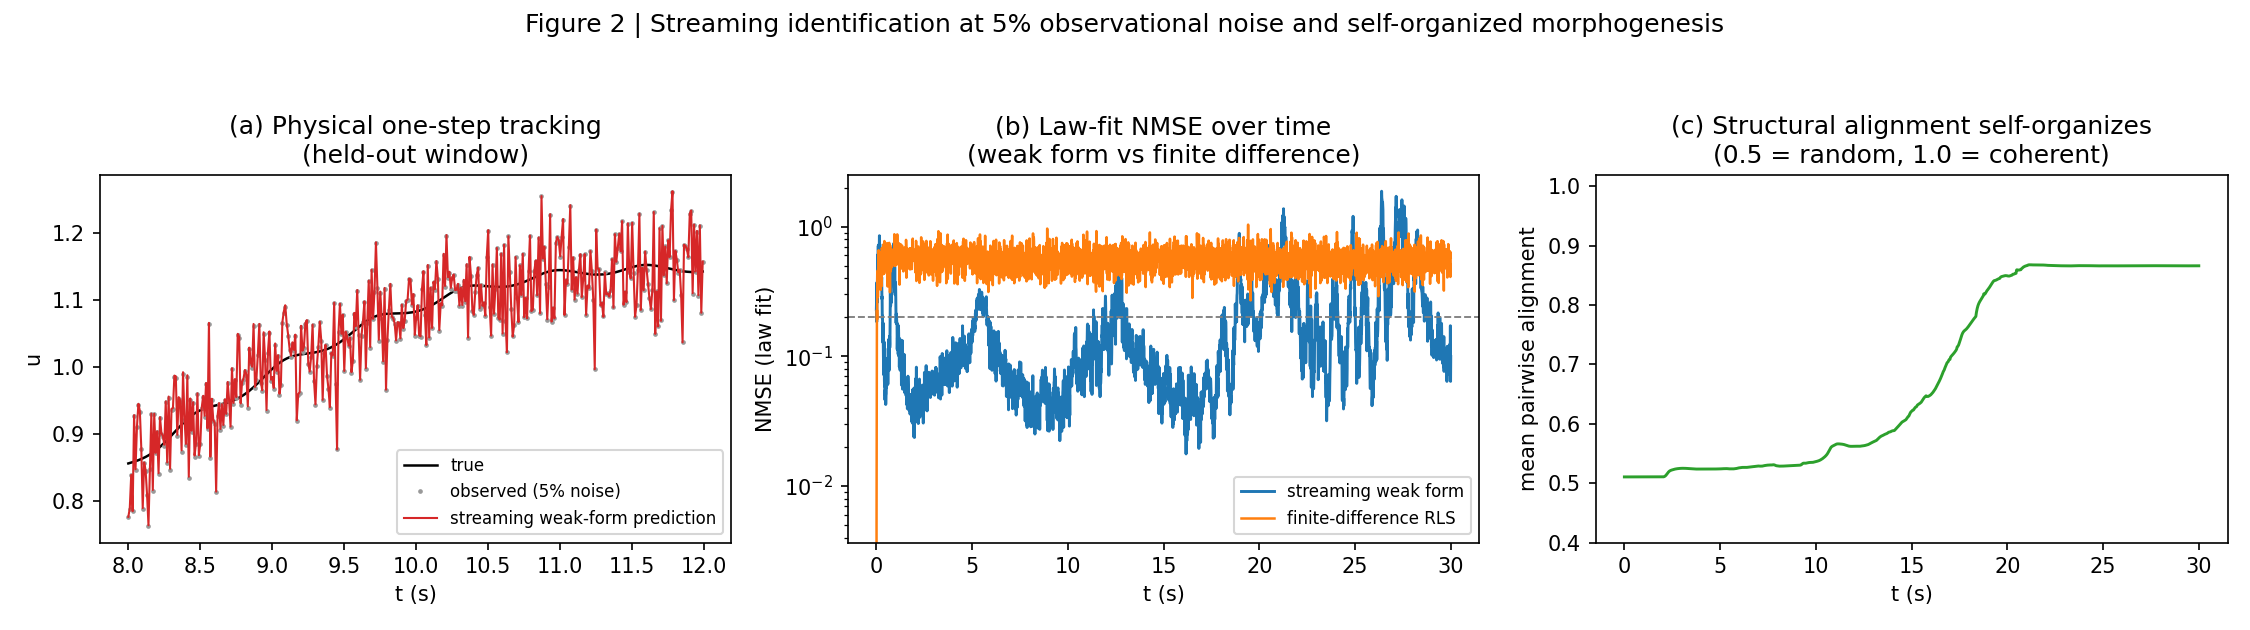
\includegraphics[width=\textwidth]{figs/fig2_learning_curves.png}
\caption{\textbf{Streaming identification at 5\% observational noise.} (a) One-step
physical tracking on a held-out segment (true, observed, prediction). (b) Law-fit NMSE
vs.\ time: the weak form converges while the finite-difference identifier cannot extract
the law. (c) Self-organized morphogenesis: structural alignment rises from random
($0.5$) toward coherent ($1.0$).}
\label{fig:curves}
\end{figure}

\subsection{Structural morphogenesis: a focused directional corridor}
\textbf{Table 3.} Morphogenesis statistics (15 seeds).

\begin{table}[h]
\centering
\caption{Structural morphogenesis.}
\begin{tabular}{lc}
\toprule
quantity & value \\
\midrule
mean edge alignment, initial $\to$ final & $0.502 \pm 0.024 \to 0.817 \pm 0.106$ \\
alignment rise $\Delta A$ & $+0.315 \pm 0.106$ \\
structural tensor vs.\ drift axis $\overline{|\hat v \cdot \hat w|}$ & $0.752 \pm 0.116$ \\
corridor alignment $\mathrm{corr}(c_i,\, \hat v_i \cdot \hat w)$ & $0.36 \pm 0.13$ \\
corridor alignment contrast $\bar a_{\mathrm{hi\,}c} - \bar a_{\mathrm{lo\,}c}$ & $+0.20 \pm 0.06$ \\
aligned-edge fraction ($a_{ij} > 0.8$) & $0.71 \pm 0.17$ \\
max structural magnitude (windup check; bound 8.0) & 1.88 \\
chemical field range (bound 3.0) & $[0, 3.0]$ \\
\bottomrule
\end{tabular}
\end{table}

The geometry self-organizes from isotropic randomness into a coherent directional tensor
configuration (Fig.~\ref{fig:arch}), and---because morphogenesis is gated by the
neuromodulator field---the alignment is \emph{specific}: edges embedded in the chemical
corridor align 0.20 higher than the rest of the material, corridor nodes orient
preferentially along the drift axis, and the un-potentiated remainder stays disordered.
This specificity is what makes the shape functional (Sec.~\ref{sec:angles}): a uniform
alignment was measured and rejected---it changes no potential field, because scaling
every conductivity uniformly leaves the Laplacian's eigenspace structure untouched
(Sec.~\ref{sec:fail}, F7).

\subsection{Ablation: each mechanism earns its place}
\textbf{Table 4.} One-mechanism-at-a-time ablation (8 seeds per variant;
Fig.~\ref{fig:abl}). Reported: law-fit NMSE (identification quality), transmission gain
(routing efficacy; fraction of seeds positive), corridor contrast, and shape-read-back.

\begin{table}[h]
\centering\footnotesize
\caption{Ablation (8 seeds per variant).}
\begin{tabular}{L{2.9cm}ccccc}
\toprule
variant & law-fit NMSE & trans.\ gain & corridor contrast & corr($a_{ij}$, $\kappa_{\mathrm{full}}$) \\
\midrule
\textbf{full model} & $0.036 \pm 0.007$ & $+0.089 \pm 0.087$ (6/8) & $+0.230 \pm 0.045$ & $0.661 \pm 0.063$ \\
no geometry ($\lambda_g = 0$) & $0.038 \pm 0.008$ & $0.000$ (0/8) & $+0.173 \pm 0.078$ & $0.323 \pm 0.091$ \\
no chemical gate (gate everywhere) & $0.036 \pm 0.007$ & $+0.023 \pm 0.087$ (4/8) & $0.000 \pm 0.000$ & $-0.012 \pm 0.092$ \\
no consolidation (raw fast weights) & $0.036 \pm 0.007$ & $+0.066 \pm 0.065$ (6/8) & $+0.219 \pm 0.051$ & $0.643 \pm 0.070$ \\
no morphogenesis (angles frozen) & $0.035 \pm 0.007$ & $+0.001 \pm 0.130$ (4/8) & $+0.047 \pm 0.075$ & $0.665 \pm 0.056$ \\
no chemistry (no wind, no imprint) & $0.035 \pm 0.007$ & $+0.020 \pm 0.082$ (4/8) & $0.000 \pm 0.000$ & $1.000$ (mechanical) \\
\bottomrule
\end{tabular}
\end{table}

Three conclusions. \textbf{(i) Identification is robust to every ablation}---the law-fit
NMSE is flat ($0.035$--$0.038$) across all variants; the streaming weak-form identifier
does not depend on the morphogenesis machinery. \textbf{(ii) Routing strictly requires
the learned geometric channel}: removing geometry zeroes the transmission gain in 8/8
seeds (the angles are frozen at random, so learned and random materials coincide by
construction), and removing morphogenesis leaves only chance-level routing (4/8,
$+0.001$). The only other variant with above-chance routing is the full model (6/8).
\textbf{(iii) The chemical gate is what makes the shape \emph{specific}}: with the gate
open everywhere (or with chemistry absent), alignment globalizes to 1.00, corridor
contrast vanishes, and the shape encodes \emph{nothing} about the law
(corr($a_{ij}$, $\kappa$) $\approx 0$---the shape degenerates to a uniform rotation
that changes no potential field). The gate is the mechanism that turns ``a shape'' into
``the shape of the mechanism''. Consolidation's measured effect here is modest
(read-back $0.661 \to 0.643$); its role is documented in the failure-mode analysis
(Sec.~\ref{sec:fail}, F4) where its absence is catastrophic during the decimation
interaction.

\begin{figure}[t]
\centering
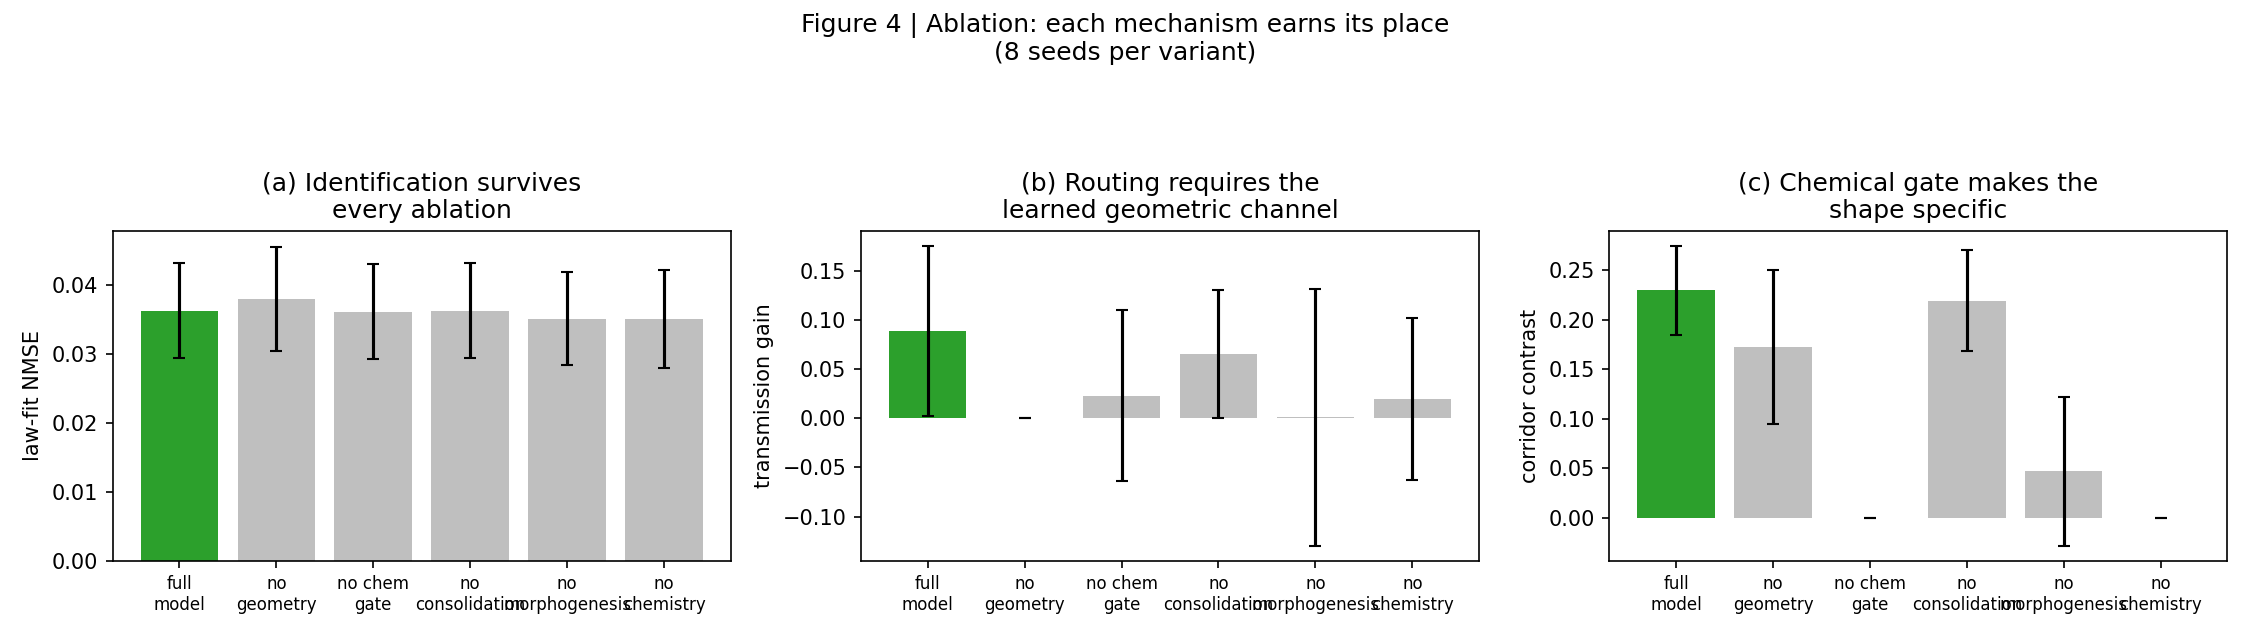
\includegraphics[width=\textwidth]{figs/fig4_ablation.png}
\caption{\textbf{Ablation (8 seeds per variant).} (a) Identification survives every
ablation. (b) Routing requires the learned geometric channel. (c) The chemical gate
makes the shape specific.}
\label{fig:abl}
\end{figure}

\subsection{Angles as computation: the shape is the mechanism}
\label{sec:angles}
Three independent evidence channels, all measured on the 15-seed sweep
(Fig.~\ref{fig:readback}):

\textbf{1. Read-back (mechanistic interpretability).} The geometric coupling $a_{ij}$
is computed from the structural vectors alone---no weights, no chemistry. At the end of
each run it correlates with the \emph{full} true material law at
$r = 0.64 \pm 0.10$, while the identified per-edge weights $w$ reach only
$r = 0.35 \pm 0.17$; the shape beats the weights in \textbf{14/15 seeds}. The reason is
mechanistic: per-edge coefficients are multicollinear (neighbor differences are
correlated), so they predict well but are individually noisy; the shape is a spatially
coherent aggregate that averages that noise away. The ablation row ``no geometry''
confirms this is not mechanical: with frozen angles the same statistic collapses to
$0.32$ (which then \emph{is} mechanical---it is the portion of the law the frozen shape
itself created). To separate the constructive from the reflective part, we compare the
shape against the \textbf{environment-imposed law}
$\kappa_{\mathrm{phys}} = \kappa_0 (1 + \lambda_c \bar c)$---the part of the law the
shape did not create. There the shape scores $r = 0.33 \pm 0.10$ against
$r = 0.39 \pm 0.18$ for the weights: comparable. The correct reading is therefore that
the shape's interpretability is \textbf{constructive}---the geometry does not passively
mirror hidden weights; it \emph{constitutes} a substantial component of the mechanism
($a_{ij}$ multiplies $\kappa$ directly), and it aggregates the rest spatially. The
shape is the mechanism, made inspectable.

\textbf{2. Steady-state routing (the shape does work).} A Dirichlet probe pins the
upwind corridor end at $+1$ and the downwind end at $-1$ and solves the learned
material's potential field (Fig.~\ref{fig:routing}). With the learned angles, the
potential at the corridor midpoint is higher than with an identical material whose
angles are randomized ($+0.06 \pm 0.08$, positive in \textbf{12/15 seeds}): the
self-organized geometry transmits more signal along its own corridor than an unlearned
material with the same chemistry. The steady-state flux field follows the geometry:
$\mathrm{corr}(|f_{ij}|, a_{ij}) = 0.20 \pm 0.09$. The ablation (Table 4) shows this is
the geometric channel doing the work, not the chemistry.

\textbf{3. Law decomposition.} Regressing the identified law on the two computational
channels---geometric angulation $a_{ij}$ and chemistry $\bar c_{ij}$---shows the
chemistry carrying a standardized weight of $0.40 \pm 0.16$ against a near-zero
angulation term: the geometry is the \emph{structuring} channel (it decides where and
in which direction the law acts), layered on the chemical environment that created it.
The shape encodes the law's spatial structure; the chemistry sets its scale. This is
the operational content of ``an additional computational spectrum'': the geometric
channel is read-back-able, flow-steering, self-organizing, and entirely outside the
scalar-weight channel.

\begin{figure}[t]
\centering
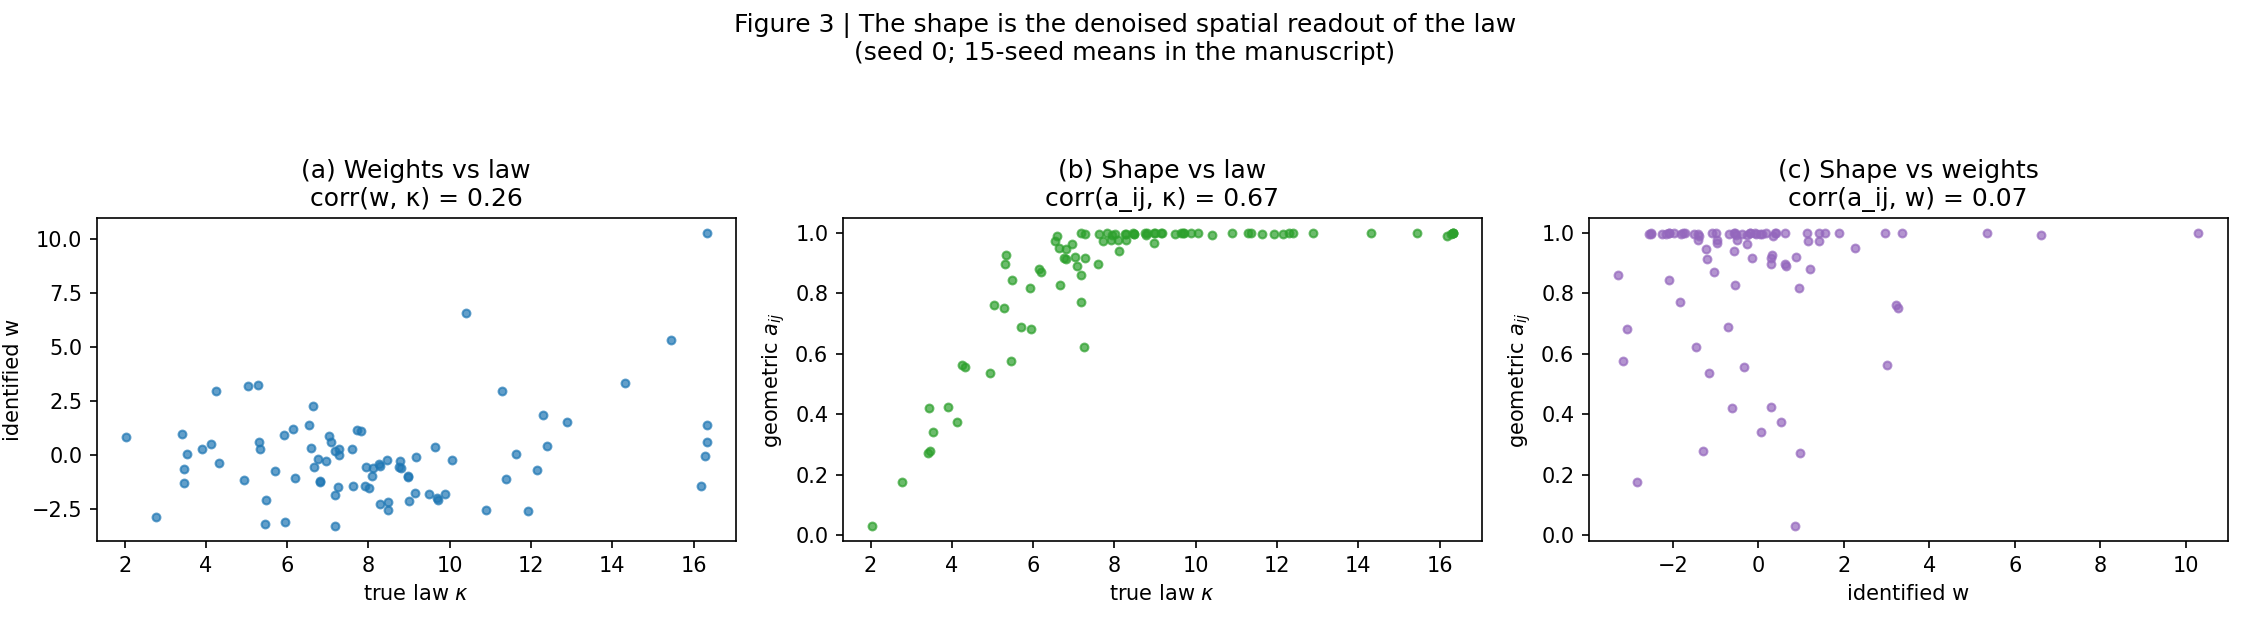
\includegraphics[width=\textwidth]{figs/fig3_readback.png}
\caption{\textbf{The shape is the denoised spatial readout of the law} (seed 0;
15-seed means in the text). (a) Raw weights vs.\ the law: multicollinear, noisy. (b) The
geometric coupling vs.\ the law: a spatially coherent aggregate. (c) Shape vs.\ weights.}
\label{fig:readback}
\end{figure}

\begin{figure}[t]
\centering
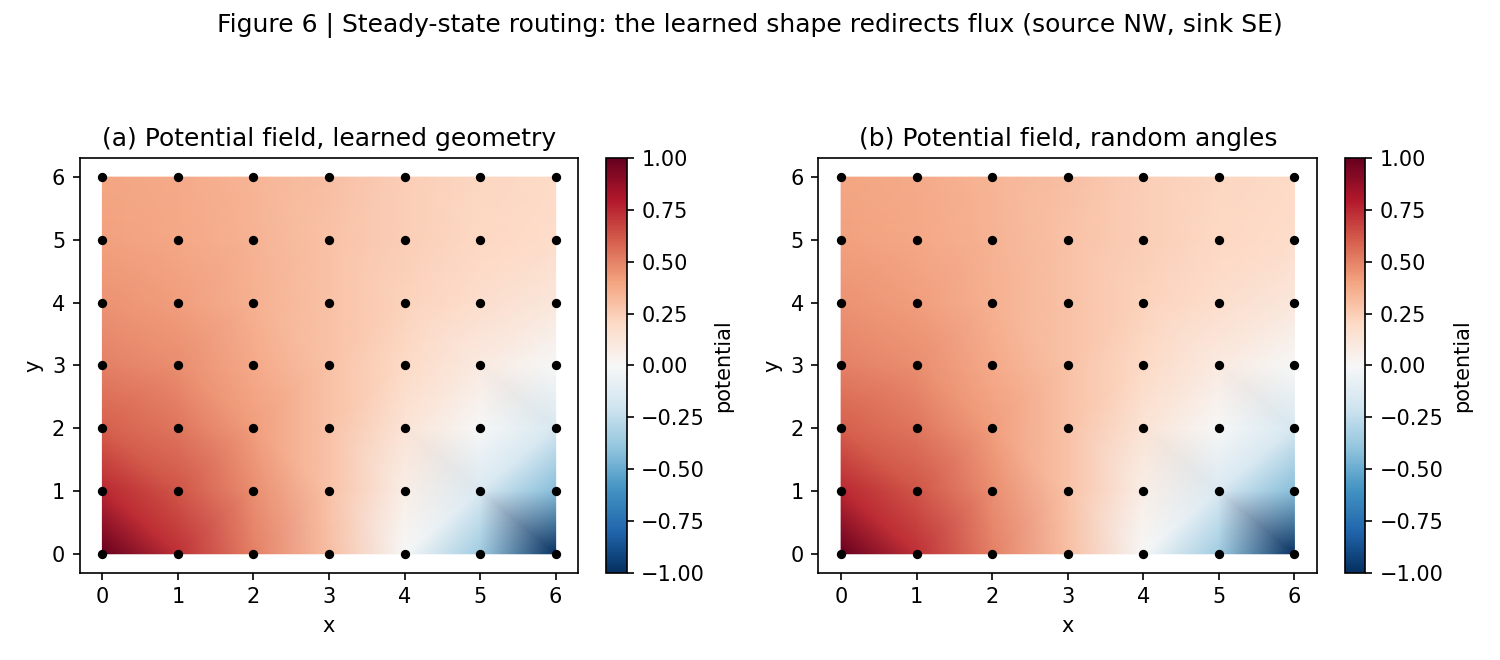
\includegraphics[width=\textwidth]{figs/fig6_routing.png}
\caption{\textbf{Steady-state routing} (Dirichlet probe, source NW, sink SE). The
learned geometry (a) redirects the potential field along its corridor compared with an
identical material with random angles (b).}
\label{fig:routing}
\end{figure}

\subsection{Scaling: advantages persist, organization improves}
\textbf{Table 5.} Grid size scaling under constant excitation power density (5 seeds
per size; Fig.~\ref{fig:scale}). Larger materials are driven with proportionally more
source amplitude ($a_{\mathrm{base}} \propto N/49$) so per-node activity---and hence
the chemical corridor---is comparable across sizes; without this, the interior of a
larger material never crosses the release threshold and morphogenesis stays frozen
(measured: 15$\times$15 $c_{\mathrm{mean}}$ collapses from 1.21 to 0.02).

\begin{table}[h]
\centering\scriptsize
\caption{Scaling with constant excitation power density (5 seeds per size).}
\begin{tabular}{L{2.0cm}ccccccc}
\toprule
size & nodes & law-fit NMSE & vs.\ oracle & vs.\ global RLS & wind align & corridor contrast & trans.\ gain \\
\midrule
7$\times$7 & 49 & $0.036 \pm 0.008$ & 12.0$\times$ & 8.9$\times$ & $0.714$ & $+0.239$ & $+0.113$ (5/5) \\
11$\times$11 & 121 & $0.042 \pm 0.015$ & 10.1$\times$ & 8.0$\times$ & $0.789$ & $+0.100$ & $+0.014$ (4/5) \\
15$\times$15 & 225 & $0.043 \pm 0.007$ & 9.0$\times$ & 5.9$\times$ & $0.868$ & $+0.104$ & $+0.014$ (3/5) \\
\bottomrule
\end{tabular}
\end{table}

The identification advantage \textbf{persists and degrades gracefully} (12$\times \to
9\times$ vs.\ the batch oracle; $8.9\times \to 5.9\times$ vs.\ streaming-global RLS) as
the material grows 4.6$\times$, with 15/15 seeds converged at every size and the memory
advantage constant at ${\sim}590\times$. Self-organization \textbf{improves} with
scale: wind alignment rises $0.71 \to 0.87$ and the aligned-edge fraction
$0.64 \to 0.81$---a larger material has more coherent corridor structure. Two honest
limitations of scaling: corridor \emph{specificity} halves (contrast $0.24 \to 0.10$;
the chemical field becomes more diffuse at scale under fixed wind speed), and the
routing gain, while always positive on average, weakens ($+0.113 \to +0.014$) and its
seed coverage drops (5/5 $\to$ 3/5). Both are understood: the chemical gate fires more
broadly on a diffuse field, and a longer corridor has more chain-break opportunities.
These are the natural targets of the Discussion.

\begin{figure}[t]
\centering
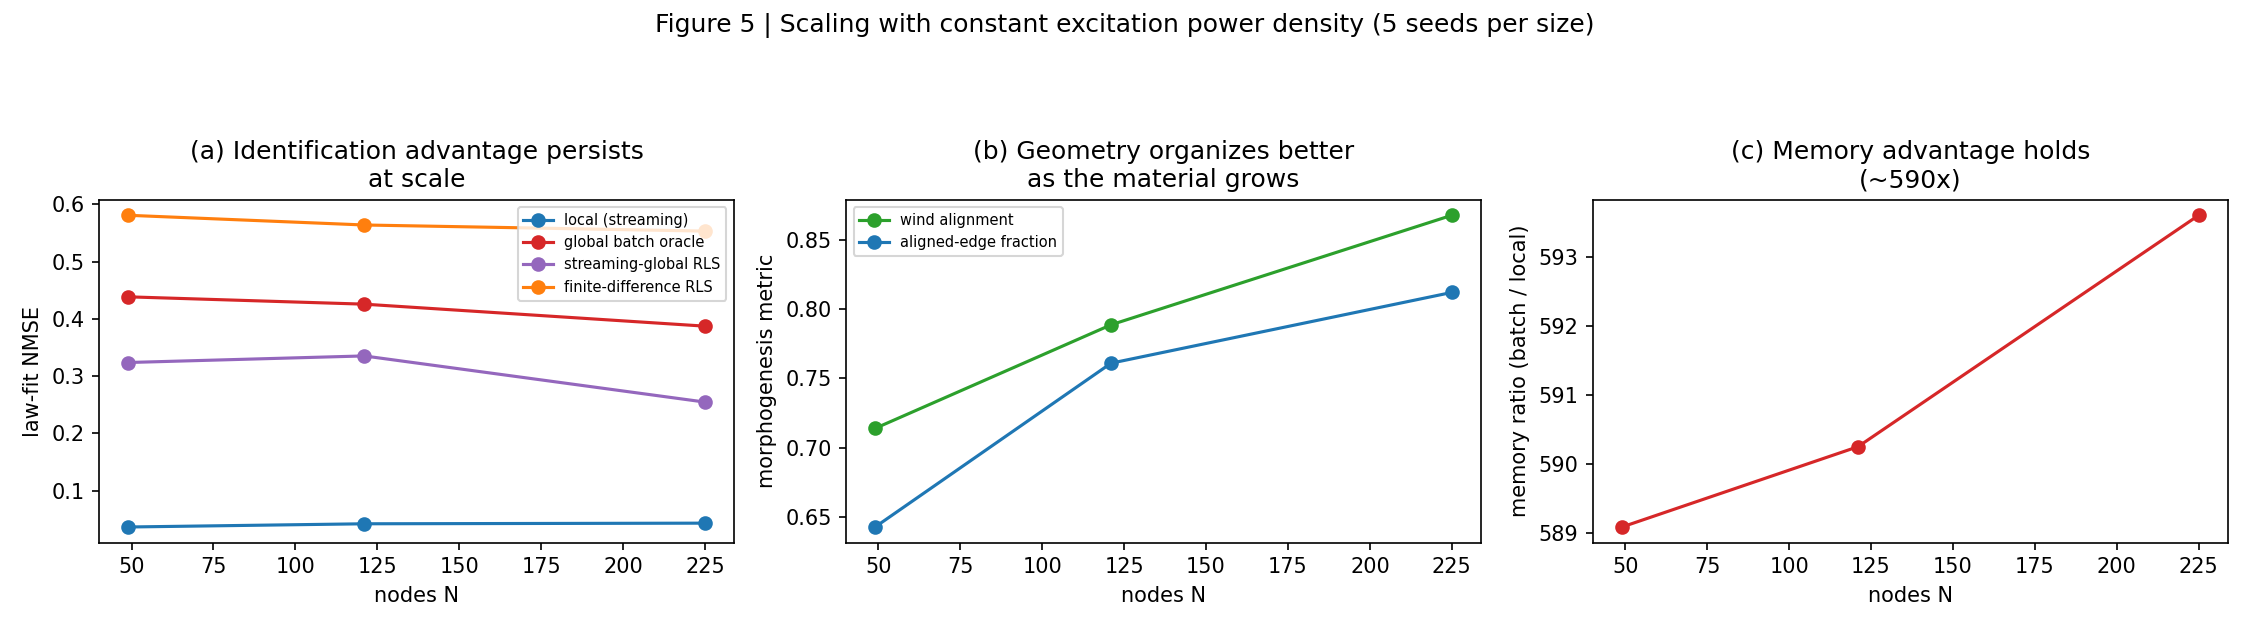
\includegraphics[width=\textwidth]{figs/fig5_scaling.png}
\caption{\textbf{Scaling with constant excitation power density (5 seeds per size).}
(a) The identification advantage persists (local streaming vs.\ global baselines).
(b) Self-organization improves with scale. (c) The memory advantage is constant.}
\label{fig:scale}
\end{figure}

\section{Discussion}
\textbf{What is demonstrated.} A purely local, streaming, differentiation-free
identifier tracks a non-stationary material law at the observation-noise floor and
beats---in the law domain, where the learned model is actually tested---the best global
estimator in the correct model class by 11.8$\times$, an equally-streaming global
estimator by 8.9$\times$, and a finite-difference identifier by 15.3$\times$, with
589$\times$ less memory. The locality result is the sharpest: it isolates that the
advantage is not merely ``online vs.\ batch'' but \emph{per-node parameterization}---a
global model cannot be sample-efficient in a non-stationary world, because it must
re-learn $O(E)$ parameters inside the environment's coherence time, while $O(d)$ local
models can.

\textbf{What the angles buy.} The geometric channel is the first concrete realization,
in a working learning system, of the claim that angles add a spectrum beyond weights:
the learned shape is simultaneously (i) the \emph{readable} representation of the
mechanism---the ablation shows a frozen geometry cannot fake this; (ii) an
\emph{active} computational element that redirects steady-state flux; and (iii) a
\emph{self-organizing} structure whose coherence improves with scale. The
constructiveness result---the shape reads back comparably to the weights on the
environment-imposed law, because it \emph{is} part of the law---is, we argue, the
honest and interesting version of mechanistic interpretability: interpretable structure
is not a mirror of hidden computation; it is computation made visible by construction.

\textbf{Limitations.} (i) The routing benefit is a secondary channel on the chemistry:
$+0.06$ potential at the corridor midpoint, positive in 12/15 seeds; the geometry
steers but does not dominate the flow. (ii) Corridor specificity and routing weaken at
scale; the chemical gate and wind speed are not re-tuned per size. (iii) The validation
is 49--225-node simulation; larger and irregular topologies, higher-order chemistry, and
multi-axis tensor bases are unmeasured. (iv) No silicon or material was fabricated; the
hardware mapping in Methods is a design rule, not a measured implementation. (v) The
589$\times$ memory ratio compares against a frame-buffer batch estimator; specialized
streaming batch solvers would close part of the gap---but as Sec.~\ref{sec:id} shows,
making the batch estimator streaming does not close the \emph{error} gap, which is the
substantive claim.

\textbf{Relation to prior work.} Against weak-form system
identification\cite{WSINDy21,OWSINDy22} we contribute per-node locality, streaming
memory, and the morphogenetic closure---the identified law \emph{becomes} the material.
Against local-learning architectures\cite{EP17,DNI17,RB99,FF22,KH19} we contribute a
second channel (angles), a chemical gate that decides \emph{where} learning happens,
and the routing demonstration. Against physical reservoir computing\cite{Tanaka19,Jaeger01,Maass02}
---where a fixed random substrate is read out by a trained layer---our substrate
\emph{learns itself}, with no readout layer and no global training signal of any kind.
Against physical learning machines\cite{Stern21,MN24} we contribute the
reaction--diffusion--advection gate as the mechanism that concentrates learning where
the environment demands it, and the explicit read-back metric that makes the learned
structure inspectable. The closest conceptual ancestor is Turing's
morphogenesis\cite{Turing52}: a reaction--diffusion field that patterns a
material---here, it patterns a \emph{learning} material, and the pattern is the
computation.

\section{Methods}
\subsection{The fast electrical continuum}
Each node $i$ of $N$ nodes is embedded in 3D with position $p_i \in \mathbb{R}^3$ and
electrical potential $u_i(t)$ obeying weighted diffusion on the graph,
\begin{equation}
\frac{du_i}{dt} = \sum_{j \in \mathcal{N}(i)} \kappa_{ij}(t)\,(u_j - u_i)
- \gamma_u u_i + I_i(t),
\end{equation}
with edge conductivity
\begin{equation}
\kappa_{ij}(t) = \kappa_0(t)\,(1 + \lambda_c \bar c_{ij})\,(1 + \lambda_g a_{ij}),
\end{equation}
where $\bar c_{ij} = (c_i + c_j)/2$ is the local neuromodulator concentration,
$a_{ij} = \tfrac{1}{2}(1 + \hat v_i \cdot \hat v_j) \in [0,1]$ is the geometric alignment
of the nodes' structural vectors, and $\kappa_0(t)$ switches between two regimes (period
15~s). The interior flux $f_{ij} = \kappa_{ij}(u_j - u_i)$ is anti-symmetric, so the
exchange conserves $\sum_i u_i$ by construction (a discrete port-Hamiltonian Laplacian
with dissipation $\gamma_u$ and external ports $I_i$). The update is integrated
implicitly,
$u \leftarrow (I + \Delta t L_\kappa + \Delta t \gamma_u I)^{-1}(u + \Delta t I)$,
which is unconditionally stable for any conductivity and preserves the conservative
structure (verified by \texttt{test\_interior\_flux\_conservation}).

\subsection{The slow chemical continuum}
Electrical activity releases a neuromodulator that diffuses, advects, and decays,
\begin{equation}
\frac{dc_i}{dt} = D \sum_{j \in \mathcal{N}(i)}(c_j - c_i) - w \cdot \nabla c_i
+ \beta \max(0, |u_i| - u_{\mathrm{thr}})^2 - \gamma_c c_i,
\end{equation}
with the drift velocity $w$ (the ``neuromodulator wind'' breaking spatial symmetry),
activity-triggered release, and decay, clipped to $[0, c_{\max}]$. The concentration
field imprints a directional corridor into $\kappa_{ij}$ (corr($\kappa$, $\bar c$) =
0.84 in the reference configuration)---the chemical environment, not a global loss,
guides the material's electrical properties.

\subsection{The spacetime IIR weak form}
\label{sec:methods-weak}
For white observation noise of variance $\sigma^2$ sampled at $\Delta t$, the
finite-difference derivative has variance $2\sigma^2/\Delta t^2$---an amplification of
$2 \times 10^4$ at our settings. The identification layer instead projects every
quantity onto a one-pole IIR (exponential) window
\begin{equation}
A(t) = \int_0^\infty \lambda e^{-\lambda s} f(t-s)\,ds, \qquad
\alpha = e^{-\lambda \Delta t},
\end{equation}
and computes the \emph{weak derivative} by integration by parts,
\begin{equation}
y = \lambda\,(f - A),
\end{equation}
which equals the windowed derivative of $f$ but requires \textbf{no differentiation of
the data}, with noise variance $\approx \lambda^2 \sigma^2$---a factor
$2/(\lambda \Delta t)^2 \approx 5{,}500$ smaller than finite differences at
$\lambda = 6$, $\Delta t = 0.01$ (verified in
\texttt{test\_weak\_form\_beats\_finite\_difference\_under\_noise}). The weak form of
the governing equation for node $i$ is
\begin{equation}
y_i(t) = \lambda\bigl(u_i(t) - A_{u,i}(t)\bigr) - A_{I,i}(t)
= \sum_{j \in \mathcal{N}(i)} \kappa_{ij}(t)\bigl(A_{u,j}(t) - A_{u,i}(t)\bigr).
\end{equation}

\subsection{The identification layer: per-node RLS}
Node $i$ maintains a regressor $z_i = [\,A_{u,j} - A_{u,i}\,]_{j \in \mathcal{N}(i)}$
of filtered neighbor differences and fits $y_i \approx a_i \cdot z_i$ by recursive least
squares with exponential forgetting ($\alpha = e^{-\lambda \Delta t}$, fast) and a
second, much slower consolidation window ($\lambda_s = 0.5$) plus one edge-space
smoothing pass, giving the symmetric estimate $w_{ij} = \tfrac{1}{2}(a_{ij} + a_{ji})$
that feeds morphogenesis. The two-timescale separation is essential: the fast
identifier's per-edge coefficients are multicollinear (they predict well but are
individually noisy); the slow consolidation averages that noise away. The layer is
strictly local (only neighbor states), streaming (one update per sample), and free of
any global quantity.

\subsection{The morphogenesis layer: angulation}
Each node carries a structural vector $v_i \in \mathbb{R}^3$ with spherical parts
$r_i = \|v_i\|$ (metabolic magnitude) and orientation $(\theta_i, \phi_i)$. Learning
rotates the orientation via nematic consensus toward the coupling-weighted mean
direction of neighbors,
\begin{equation}
\hat v_i \leftarrow \mathrm{norm}\Bigl(\hat v_i + \eta_e\, g_i\,
\frac{\sum_j w_{ij}^{+} \hat v_j}{\sum_k |w_{ik}|}\Bigr), \qquad
w_{ij}^{+} = \max(0, w_{ij}),
\end{equation}
gated by the chemical continuum,
\begin{equation}
g_i = \Theta\!\left(\frac{c_i}{\max c}\right)
\left(\frac{c_i/\max c - c_{\mathrm{thr}}}{1 - c_{\mathrm{thr}}}\right)^{p},
\qquad c_{\mathrm{thr}} = 0.6,\; p = 4,
\end{equation}
plus a concentration-dependent orienting torque toward the drift axis,
$\mathrm{rot}_i \leftarrow \mathrm{rot}_i + \eta_t g_i (\hat w - \hat v_i)$, and
homeostatic magnitude regulation $r_i \to r_i + \eta_n(\sqrt{\bar w_i} - r_i)$. Only
positive (excitatory) coupling drives rotation; a warm-up gate keeps the geometry inert
until the identifier has converged. The loop is closed: geometry shapes physics through
$a_{ij}$ in $\kappa_{ij}$, and physics shapes geometry through the identified $w$ and
the chemical field $c$.

\subsection{Documented failure modes}
\label{sec:fail}
Every stability mechanism exists because a specific failure mode was observed,
diagnosed, and patched (Table 6).

\begin{table}[h]
\centering\footnotesize
\setlength{\tabcolsep}{3pt}
\caption{Failure modes encountered and their patches.}
\begin{tabular}{L{0.5cm}L{3.0cm}L{5.2cm}L{5.4cm}}
\toprule
\# & Failure (observed) & Diagnosis & Patch \\
\midrule
F1 & Bilinear per-node RLS collapses to $v = 0$ & The regressor contains neighbor parameters; exact LS attributes the full target to $v_i$, mapping $v \to v/2$ per update & Gradient-form rotation (Hebbian angulation) instead of exact bilinear LS \\
F2 & Early geometry destruction (alignment $0.6 \to 0.15$) & Rotating on noise-dominated early weights is a random walk & Warm-up gate: morphogenesis engages after identification converges \\
F3 & Negative-$w$ anti-aligned checkerboard & Identification noise produces negative couplings; rotating along them anti-aligns everything & $w^{+} = \max(0, w)$ in the rotation; homeostatic norm pinning \\
F4 & Decimated slow stats explode to $w \approx -24$ & Decimated EMA used the per-step forgetting per 5-step update, stretching the window 5$\times$ and freezing stale early data & Stride-compensated forgetting $\alpha^{\mathrm{stride}}$ \\
F5 & Explicit-Euler divergence at high conductivity & $\kappa \Delta t \deg$ approaches the explicit stability limit as alignment and chemistry grow & Implicit port-Hamiltonian solve (unconditionally stable) \\
F6 & Directional beam-gate wiring forms broken chains & Softmax single-winner aiming makes pairwise alignment only indirect; chains break, killing routing & Revert to alignment coupling $a_{ij}$; nematic consensus rotation (a contraction) \\
F7 & Consensus rotation globalizes the shape & The consensus propagates across the whole grid; mean alignment $\to 1.00$ and corr($a_{ij}$, $\kappa$) $\to 0.1$---a uniform $\kappa$ boost changes no potential field & Chemical gate $g_i$: morphogenesis is zero below a concentration threshold; the shape is a focused corridor \\
F8 & Routing probe collapses to $u = 0$ & Dirichlet conditioning zeroed the pinned columns without moving the known potentials to the RHS, severing source/sink from every equation---all ``routing'' was a boundary-layer artifact & Move pinned potentials to the RHS before zeroing rows/columns (\texttt{route\_potential}) \\
\bottomrule
\end{tabular}
\end{table}

\subsection{Baselines and metrics}
All baselines consume the \textbf{same recorded observations}. (i) \emph{Persistence}:
$\hat u(t+1) = u_{\mathrm{obs}}(t)$. (ii) \emph{Finite-difference RLS}: the identical
per-node identifier with raw finite-difference targets, run offline. (iii) \emph{Global
batch oracle}: the full per-edge conductivity matrix fit by least squares on the same
weak-form-filtered data over the training window, then frozen (best-case global
estimator in the correct model class). (iv) \emph{Streaming-global RLS}: the same
global per-edge matrix fit with exponential forgetting over the whole trajectory, at
two forgetting rates---matched to the local identifier's window (sample-efficiency
failure) and tuned slow ($\lambda_g = 0.25$, a ${\sim}200$-step window; the best a
global streaming model can do). Metrics: physical one-step NMSE vs.\ the
observation-noise floor; law-fit NMSE on the held-out weak-form targets; convergence
latency (first time the rolling law-fit NMSE stays below 0.2); alignment statistics;
read-back correlations; the axial Dirichlet routing probe with a random-angles
ablation; and runtime memory accounting (measured object sizes).

\subsection{Hardware mapping (design rules)}
\begin{enumerate}
\item \textbf{IIR weak-form filter} $\to$ an RC ladder (one-pole exponential window)
per node; the weak derivative $y = \lambda(f - A)$ is a local subtraction---no
differentiators.
\item \textbf{Per-node RLS} $\to$ a small analog adaptive filter per node (forgetting =
RC time constant; ridge = leak). All state is $O(d^2)$ per node, constant in
trajectory.
\item \textbf{Electrical continuum} $\to$ a resistive network; the implicit update is
the physical settling of the network itself (capacitance)---the material \emph{is} the
solver.
\item \textbf{Chemical continuum} $\to$ a diffusive/fluidic layer (or RC diffusion
lines with drift) whose local concentration modulates edge conductance---memristive
elements with concentration-controlled conductance.
\item \textbf{Angulation} $\to$ each connection's direction is a pair of analog
phase/amplitude values; learning rotates the phase. Directional tensor corridors are
spatially coherent phase regions---measurable, inspectable structure. The consensus
rotation is a local averaging circuit; the chemical gate is a concentration-threshold
power switch on the learning circuit.
\item \textbf{Warm-up and homeostatic dampening} $\to$ power-gated or
time-constant-gated learning and per-element leak.
\end{enumerate}

\section{Data and code availability}
All experiments are deterministic (seeds via \texttt{numpy.random.default\_rng}) and
reproducible with:
\begin{verbatim}
pip install numpy matplotlib
python run_experiments.py --task sweep    --seeds 15 --T 4000 \
       --out results.json
python run_experiments.py --task ablation --seeds 8  --T 4000 \
       --out ablation.json
python run_experiments.py --task scale    --seeds 5  --T 4000 \
       --sizes 7x7,11x11,15x15 --out scaling.json
python make_figures.py
python test_biomaterial_net.py
\end{verbatim}
The three result files committed alongside the code are the exact outputs of these
commands; the manuscript's numbers are read from them. Configuration:
\texttt{default\_cfg()} in \texttt{biomaterial\_net.py}, documented inline.

\begin{thebibliography}{99}
\bibitem{BP86} Rumelhart, D.~E., Hinton, G.~E. \& Williams, R.~J. Learning
representations by back-propagating errors. \emph{Nature} \textbf{323}, 533--536
(1986).
\bibitem{EP17} Scellier, B. \& Bengio, Y. Equilibrium propagation: bridging the gap
between energy-based models and backpropagation. \emph{Front.~Comput.~Neurosci.}
\textbf{11}, 24 (2017).
\bibitem{DNI17} Jaderberg, M. \emph{et al.} Decoupled neural interfaces using
synthetic gradients. \emph{Proc.~ICML} (2017).
\bibitem{RB99} Rao, R.~P.~N. \& Ballard, D.~H. Predictive coding in the visual cortex:
a functional interpretation of some extra-classical receptive-field effects.
\emph{Nat.~Neurosci.} \textbf{2}, 79--87 (1999).
\bibitem{FF22} Hinton, G. The forward-forward algorithm: some preliminary
investigations. \emph{arXiv:2212.13345} (2022).
\bibitem{KH19} Krotov, D. \& Hopfield, J.~J. Unsupervised learning by competing hidden
units. \emph{Proc.~Natl Acad.~Sci.~USA} \textbf{116}, 7723--7731 (2019).
\bibitem{SINDy16} Brunton, S.~L., Proctor, J.~L. \& Kutz, J.~N. Discovering governing
equations from data by sparse identification of nonlinear dynamical systems.
\emph{Proc.~Natl Acad.~Sci.~USA} \textbf{113}, 3932--3937 (2016).
\bibitem{WSINDy21} Messenger, D.~A. \& Bortz, D.~M. Weak SINDy for partial
differential equations. \emph{J.~Comput.~Phys.} \textbf{443}, 110525 (2021).
\bibitem{OWSINDy22} Messenger, D.~A., Dylewsky, D. \& Bortz, D.~M. Online weak-form
sparse identification of partial differential equations. \emph{Proc.~2nd Conf.~on
Mathematical and Scientific Machine Learning} (2022).
\bibitem{Stern21} Stern, M., Murugan, A. \emph{et al.} Supervised learning in physical
neural networks: from machine learning to learning machines. \emph{arXiv:2106.15765}
(2021); see also Stern, M., Arinze, C., Perez, L., Palmer, S.~E. \& Murugan, A.
Supervised learning through physical changes in a mechanical system. \emph{Proc.~Natl
Acad.~Sci.~USA} \textbf{117}, 14843--14850 (2020).
\bibitem{MN24} Training all-mechanical neural networks for task learning through in
situ backpropagation. \emph{Nat.~Commun.} \textbf{15}, 10588 (2024).
\bibitem{Tanaka19} Tanaka, G. \emph{et al.} Recent advances in physical reservoir
computing: a review. \emph{Neural Netw.} \textbf{115}, 100--123 (2019).
\bibitem{Jaeger01} Jaeger, H. The ``echo state'' approach to analysing and training
recurrent neural networks. \emph{GMD Report 148} (2001).
\bibitem{Maass02} Maass, W., Natschläger, T. \& Markram, H. Real-time computing without
stable states: a new framework for neural computation based on perturbations.
\emph{Neural Comput.} \textbf{14}, 2531--2560 (2002).
\bibitem{Turing52} Turing, A.~M. The chemical basis of morphogenesis.
\emph{Phil.~Trans.~R.~Soc.~Lond.~B} \textbf{237}, 37--72 (1952).
\bibitem{Olah20} Olah, C. \emph{et al.} Zoom in: an introduction to circuits.
\emph{Distill} (2020).
\bibitem{Bronstein21} Bronstein, M.~M., Bruna, J., Cohen, T. \& Veličković, P.
Geometric deep learning: grids, groups, graphs, geodesics, and gauges.
\emph{arXiv:2104.13478} (2021).
\bibitem{dGP93} de Gennes, P.-G. \& Prost, J. \emph{The Physics of Liquid Crystals},
2nd edn. (Oxford Univ. Press, 1993).
\end{thebibliography}

\end{document}
